%======================================================================
\chapter{Introduction}
\label{cha:i}
%======================================================================

This introduction chapter describes the goal of my Ph.D. study: an augmented reality framework for training scenarios.
First, we depict the application scenario.
Next, the expected contributions of the proposed frameworks are listed.
Third, the missing building blocks are identified.
Last, we conclude with an outline of the manuscript structure.

\section{Overview}
\label{sec:i:ov}

Augmented Reality (AR) is attracting attention. The use of AR in numerous fields has been explored by researchers, such as games, communication, medicine, training and etc~\cite{nakajima2003,gonzalez-franco2016,hincapie2011,webel2011}.
In this article, we discuss the use of AR in training and propose a new framework that facilitates remote training.

Currently, traditional training methods (e.g. book, audio and videos) are still the most popular in remote training. However, AR systems are now widely regarded as a promising platform for complex and highly demanding tasks.
Gavish et. al. developed an experiment to evaluate the performance difference between AR training system and traditional training system~\cite{gavish2015}, by using an AR system and a traditional training system in a real industrial maintenance and assembly task. They argued that trainees using AR training system achieve fewer unsolved errors.

AR systems can be dated back to the 1960s~\cite{sutherland1968,johnson2010, yuen2011}. Boeing~\cite{caudell1992} had already used AR technology in their wire bundle assembly training. They leveraged a Head-Mounted Display (HMD) combined with head position sensing to superimpose a computer-produced diagram on real-world objects. Since then, many AR systems have been proposed and applied in training. These systems can be categorized into two categories: virtual objects and real objects. Fig.~\ref{fig:category} shows two examples, where the left one shows that a trainee is interacting with a real object, and the right one depict that a trainee is interacting with a virtual object. In this article, we are interested in the platforms in the latter category--real objects. A common feature of this type of systems is that these systems use predefined scripts and materials to show the trainees essential information or correct operation procedures superimposed on real-world objects.
Therefore, authoring tools became an important issue in AR training, since AR training applications are usually designed as task-specific, in order to be more robust.
Researchers have developed a variety of approaches to facilitate the authoring process~\cite{wang2010,petersen2012,anderson2013,bhattacharya2015}.
However, these are not real-time authoring tools, since the content need to be prepared or captured before the training.
Practical feedback solution is another popular research topic. Many AR training platforms are providing the trainees with rich and accurate information, but pay less attention on evaluating the performance of trainees. Re and Bordegoni~\cite{re2014} presented a monitor system for training, such that supervisors could check the assembly/maintenance activity from a remote display and provide feedback to the users whenever necessary. However, it does not allow gathering feedback from the trainees and correcting during the training process.

\section{Scenario}
\label{sec:i:s}

We are proposing a training system with augmented reality hardware.
We are envisioning a scenario where a factory is preparing a new assembly task.
Before actually conducting the task, all the workers must go through a training process to learn the essential knowledge needed in the task.
The trainer is in another country and will train the trainees remotely through an AR training system.
All materials that need to be prepared beforehand are the CAD models of all components of the product.
At a location in another country, the trainer assembles the product from the beginning, and the procedure is recorded by a video camera. Poses of the components of the product in each frame are calculated. The recorded procedure serves as a guide for the training.
On the other side, the trainees wear AR glasses or hold mobile devices that face the components they are assembling. What they need to do is will show on the glasses or displays as an overlay on the real object. More specifically, if a trainer guides to dock a battery onto the battery jar, a virtual battery is animated to move from the current position of the real object to the position it should be at.
For a complex assembly task, this system is able to reduce the authoring time for the guide dramatically, since the trainer does not need to write scripts or programs for the AR guide.
Moreover, the guide can be authored by the trainer during the training in real-time.
Both of the trainer and the trainees wear AR glasses or hold mobile devices, with cameras facing the components they are assembling.
Whenever the trainer assembles a component, a virtual component will show on the glasses or displays of all the trainees, and is animated to show where it should be moved to.
Similarly, the poses of the components that each trainee has moved are also recorded by the camera and calculated.
Those poses are transmitted to the trainer's glasses or mobile device and shown as virtual objects.
The virtual objects rendered for the trainees can be distinguished by labels or colors. If there are too many trainees, only those components that are assembled incorrectly are shown.

The proposed system has a wide variety of applications, especially in assembly and maintenance training and medical training.

We use two figures to depict the details of the scenario, with each of them showing one part of it.
Figure~\ref{fig:scenario1} shows how the trainer gives instructions to the trainees.
The upper part shows the setup of the trainer side. The grey gear represents the original pose of the component  \#2, while the black and oblique gear shows the pose of it after some operations.
The trainer wears augmented reality glasses that are equipped with a camera. The camera is used to capture videos and send them to the server.
The server estimates the pose of each component in every video frame it receives, with the CAD of all components known beforehand.
If the AR glasses are not available, a mobile device with a camera can be used, e.g. a mobile phone or a tablet.

\begin{figure*}
	\centering
	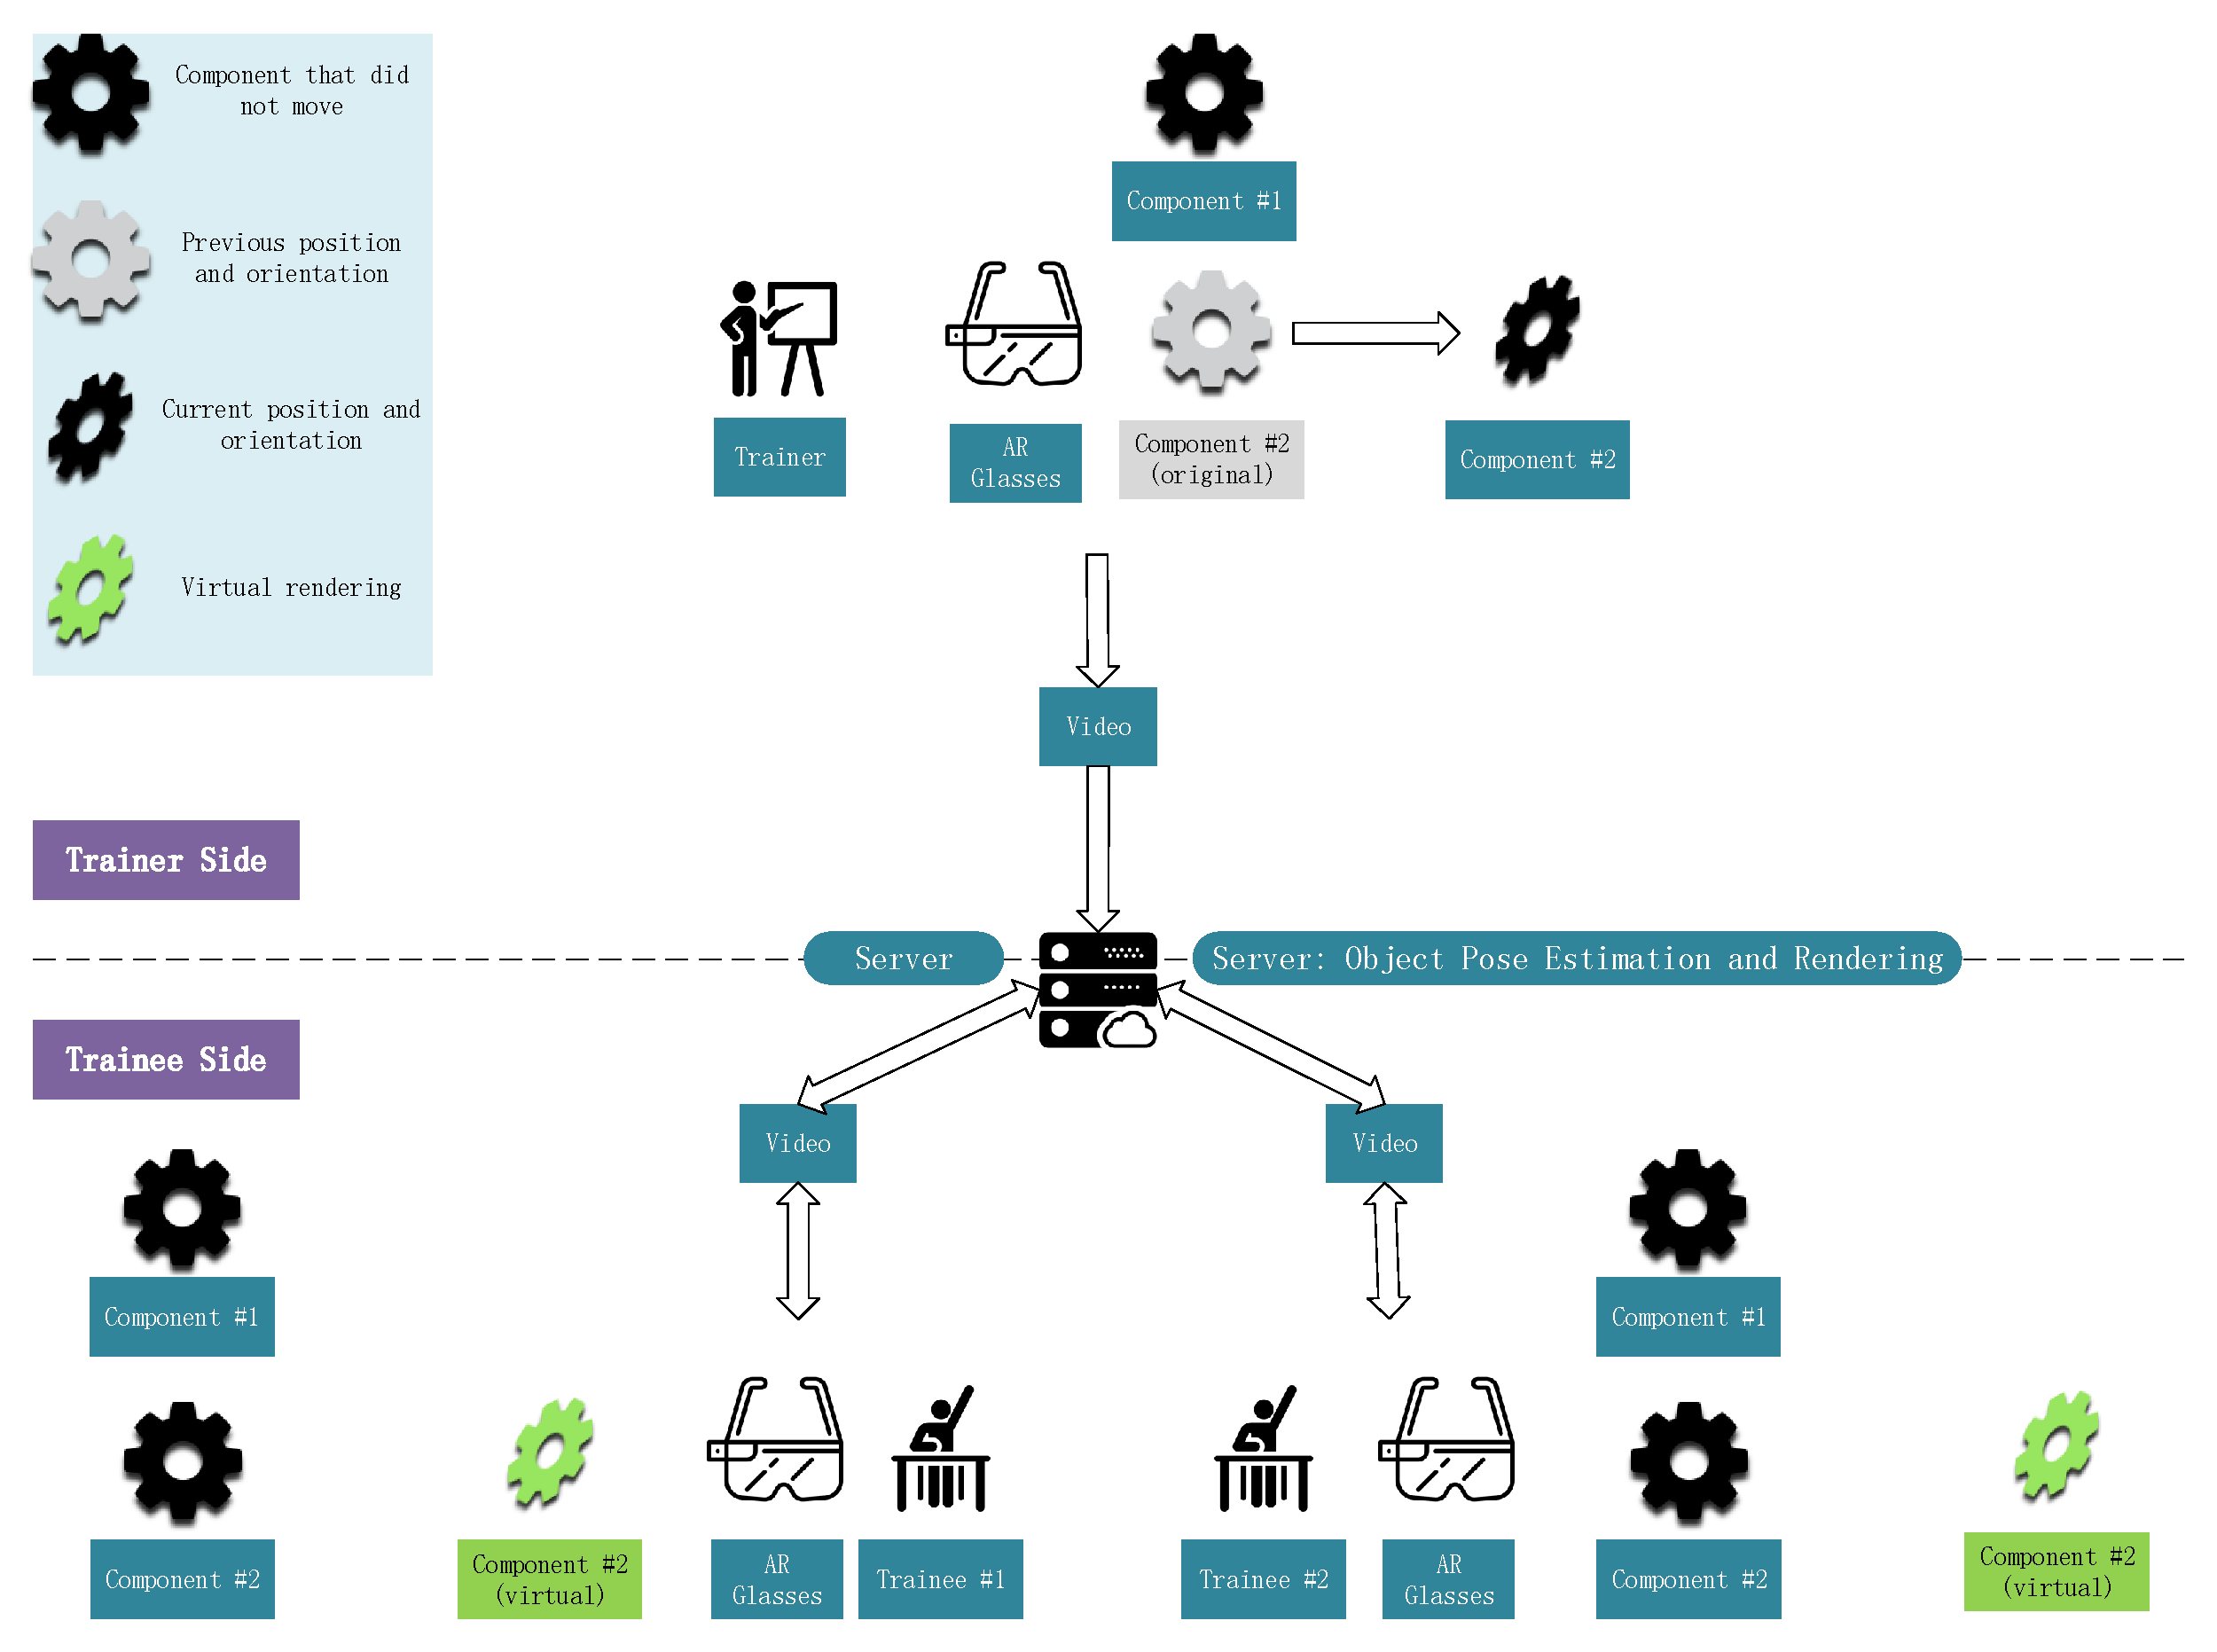
\includegraphics[width=\textwidth]{figures/scenario1.pdf}
	\caption{Training Scenario Part 1. This figure shows how the operations made by the trainer are rendered on the trainee side. The gears represent the components in the training scenario. The black gears denote the real components, while grey ones are their previous poses and the green gears demonstrate the virtual component rendered by the augmented reality devices. Moreover, the oblique gears represent the current pose after a translation and a rotation.}
	\label{fig:scenario1}
\end{figure*}

\begin{figure*}
	\centering
	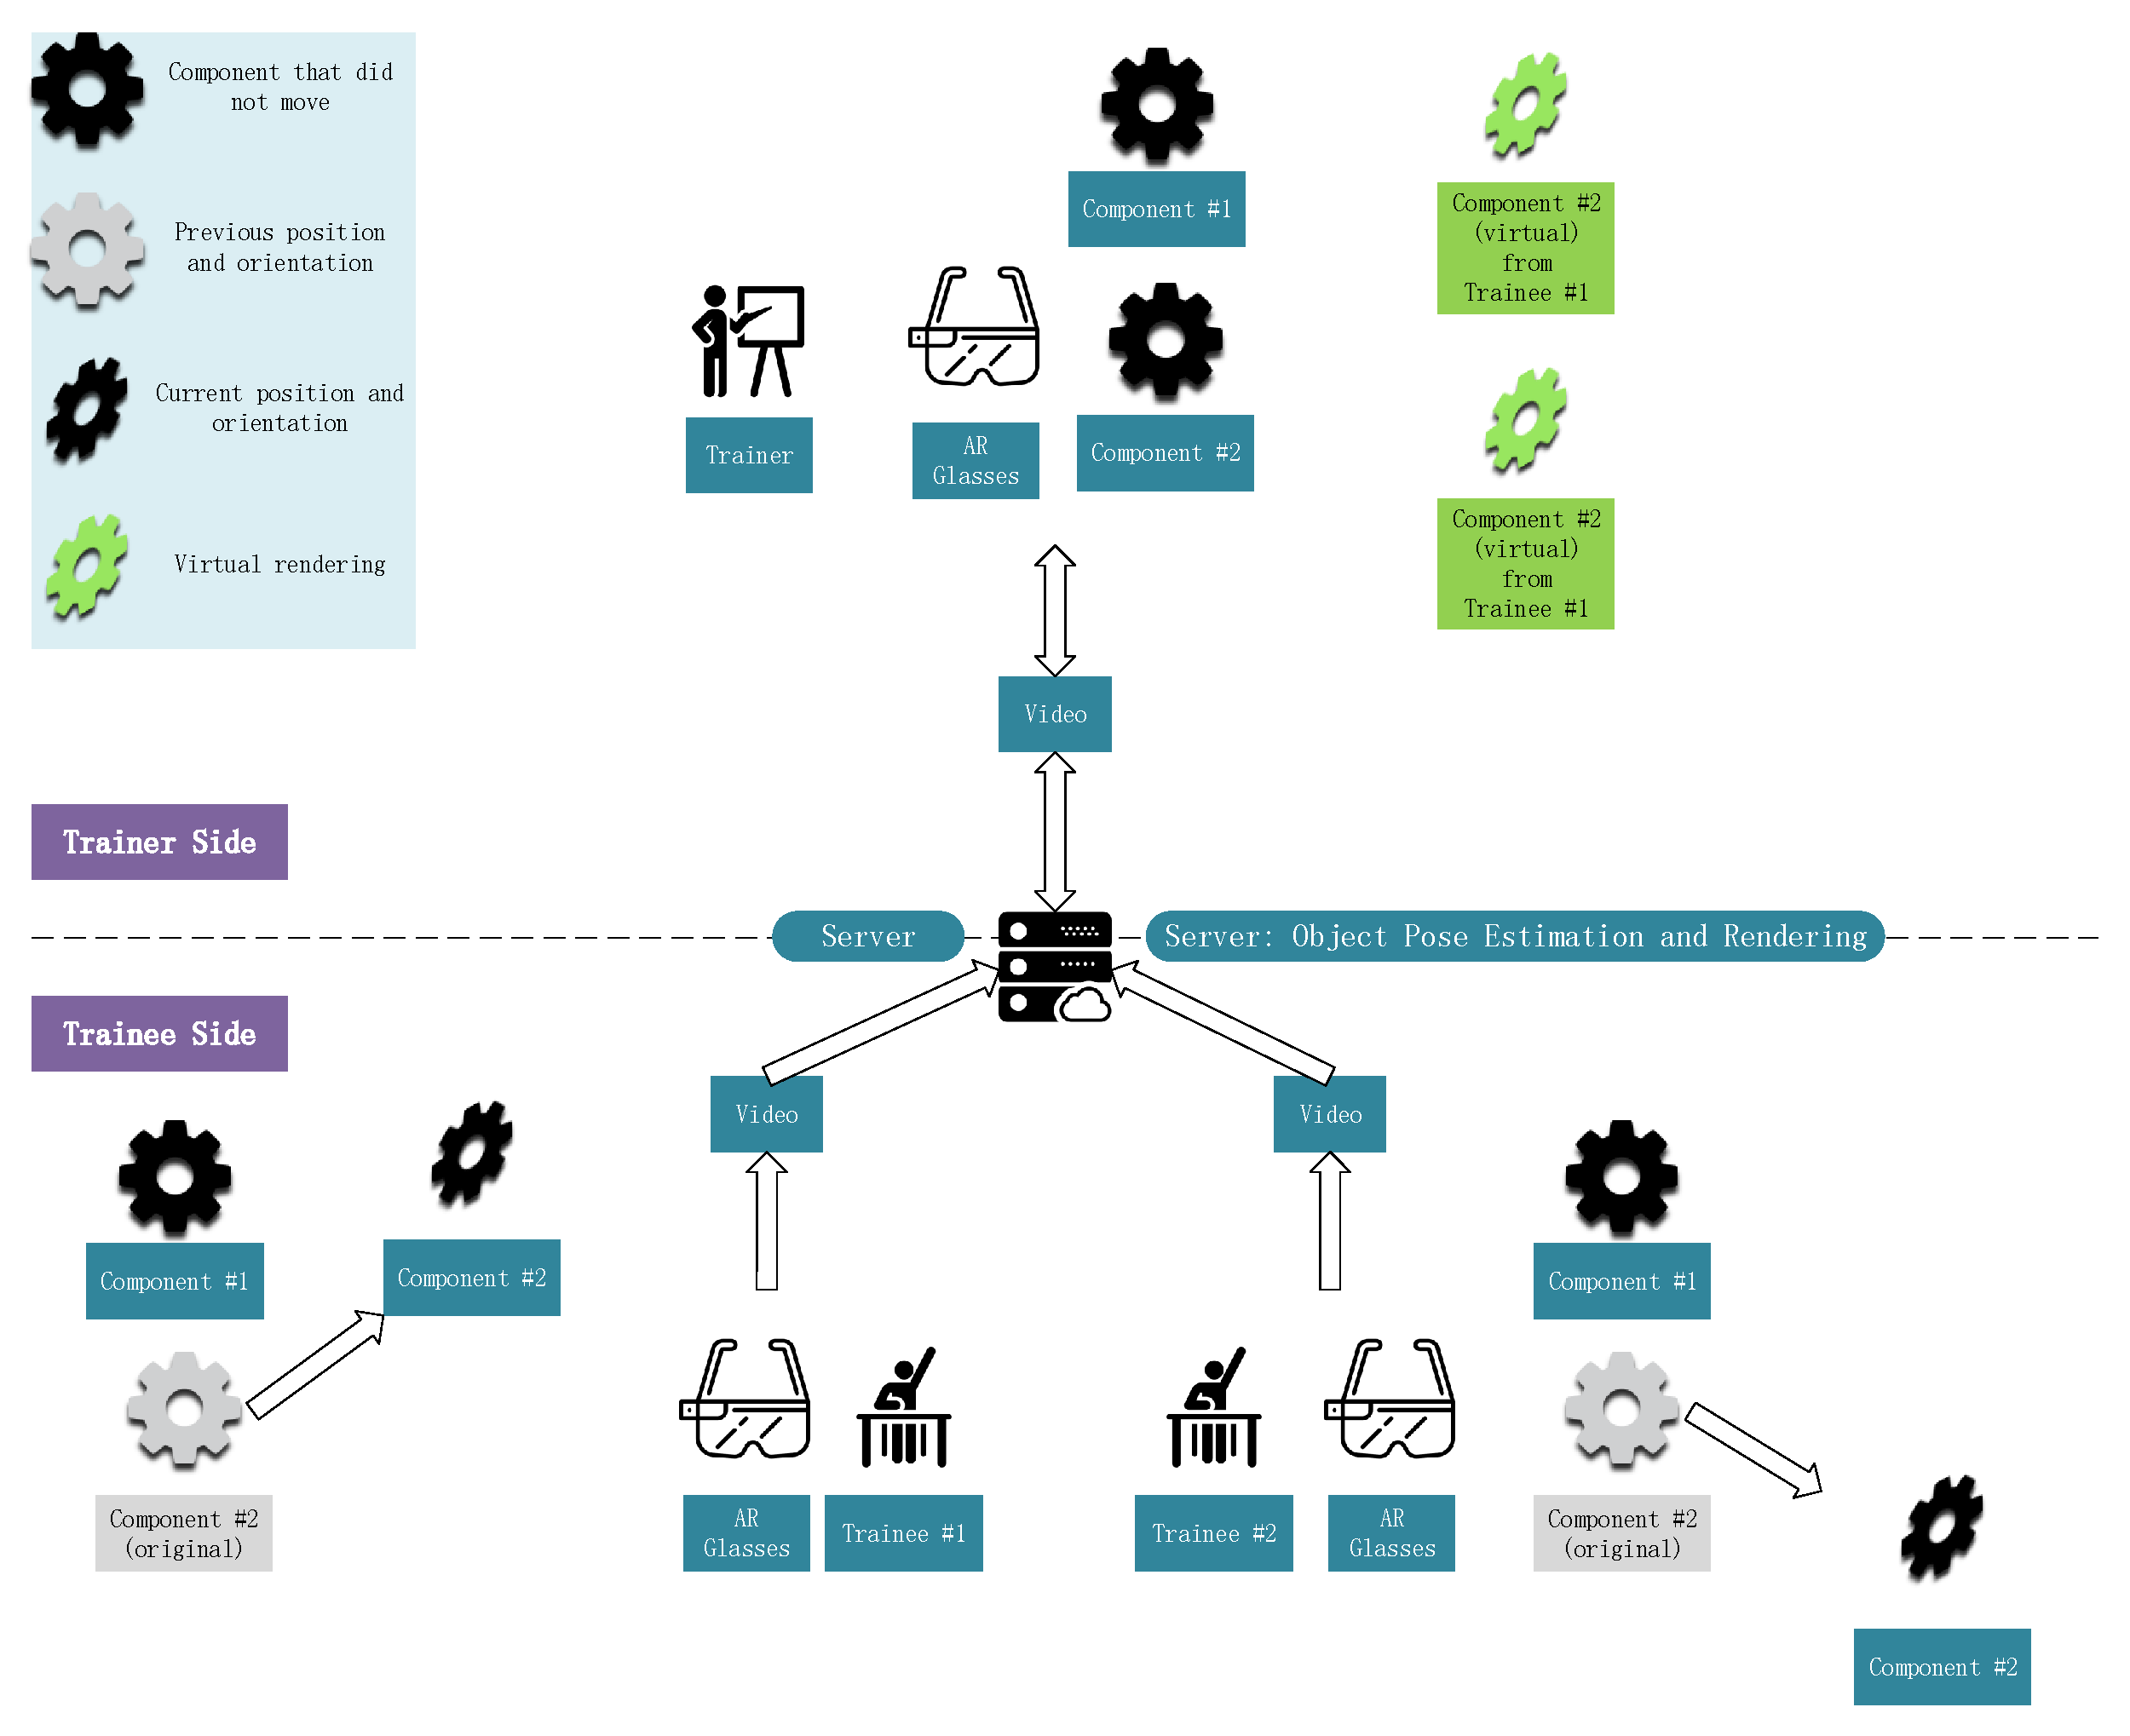
\includegraphics[width=\textwidth]{figures/scenario2.pdf}
	\caption{Training Scenario Part 2. This figure shows how the operations made by the trainees are rendered on the trainer side. The gears represent the components in the training scenario. The black gears denote the real component, while grey ones are their previous poses and the green gears demonstrate the virtual component rendered by the augmented reality devices. The oblique gears represent the current pose after a translation and a rotation.}
	\label{fig:scenario2}
\end{figure*}

The lower part of Figure~\ref{fig:scenario1} shows the setup of the trainee side.
There are same components in the training environment of each trainee as on the trainer side.
The trainees also wear augmented reality glasses.
Similar to the trainer side, the glasses are equipped with a camera that records videos and sends them to the server. With the video received from the trainee side, the server is able to calculate the pose of components related to each trainee.
As mentioned above, the server also estimates how the trainer moved every component on his or her side. Then it renders the 3D model of each component that has been moved, according to each trainee's view and sends it to the trainees' glasses as videos.
The black gears represent the real components on the trainee side, while the green gears show the changes made by trainer.

Figure~\ref{fig:scenario2} demonstrates the second part of the scenario. It shows how the trainer sees the operations made by the trainees.
After receiving instructions from the trainer, each trainee performs his or her own operations. The operations are recorded by the camera in the augmented reality glasses as a video.
Similar to the trainer side of the first part, the server estimates how each component is moving. The estimations are performed for each video from the trainees.
Moreover, the server also receives a live video from the trainer, and calculates the pose of every component on the trainer side.
Then the server renders the components according to the operations made by each trainee, sends the virtual components to the trainer and displays them with the augmented reality glasses.
Note that a trainee may behave differently from each other, so several versions of each component are sent to the trainer. As shown in Figure~\ref{fig:scenario2}, trainee \#1 moves component \#2 up, while trainee \#2 moves component \#2 down. Thus there are two versions of the virtual component shown in the trainer's view (marked green).

The components on the trainer side and the trainee side must be the same, otherwise the training makes no sense. However, they do not need to be at the same location or orientation, since the server is responsible for tracking each component on each side.

\section{Expected Contributions}
\label{sec:i:ec}

The proposed AR training framework has three main contributions.

\begin{itemize}
	\item
	We propose a method that allows the trainer to author guidances in real-time. A common feature of the existing work is that these systems use predefined scripts and materials to show the trainees essential information or correct operation procedures superimposed on real-world objects. Therefore, for a new training task, people must author the training process beforehand, which can be inconvenient, especially for complex tasks.
	\item
	We propose a method that enables the trainer to collect feedback from the trainees during the training process in real-time. Although practical feedback gathering solutions have been proposed by many researchers, they still do not allow gathering feedback from the trainees and correcting mistakes by trainees during the training process, which may improve the outcome of AR training systems.
	\item
	We propose a method that makes the AR training framework work with devices without powerful graphics capacity. Because AR training systems often rely on mobile device, no matter if they are AR glasses, mobile phones or tablets, which have very limited rendering capacity. This can influence the visual quality of the training process.
\end{itemize}

\section{Outline}
\label{sec:i:ol}

The reminder of this proposal is structured as follows: Chapter~\ref{chap:bg} reviews the literature related to augmented reality and its application in training; Chapter~\ref{chap:dm} unveils the details about the proposed method; Chapter~\ref{chap:e} describes the evaluation method that will be used to examine the effectiveness of the proposed method. Chapter~\ref{chap:vos} shows our work on video object segmentation; Chapter~\ref{chap:hrr} demonstrates our work on hybrid remote rendering; Chapter~\ref{chap:c} concludes this thesis proposal and outlines the schedule of the remaining work.
